\documentclass[10pt,aspectratio=169]{beamer}
% \documentclass[10pt,aspectratio=169,handout]{beamer}

% silence some Metropolis warnings
\usepackage{silence}
\WarningFilter{beamerthememetropolis}{You need to compile with XeLaTeX or LuaLaTeX}
\WarningFilter{latexfont}{Font shape}
\WarningFilter{latexfont}{Some font}

% define custom colors
\definecolor{dark gray}{HTML}{444444}
\definecolor{light gray}{HTML}{777777}
\definecolor{dark red}{HTML}{BB0000}
\definecolor{dark green}{HTML}{00BB00}

% configure metropolis
\usetheme[numbering=fraction]{metropolis}
\setbeamercolor{background canvas}{bg=white}
\setbeamercolor{frametitle}{bg=dark gray}
\setbeamercolor{alerted text}{fg=dark red}
\setbeamercolor{item projected}{bg=dark red}
\setbeamercolor{local structure}{fg=dark red}
\setbeamersize{text margin left=0.5cm,text margin right=0.5cm}
\setbeamercovered{transparent=10}

% use thicker lines
\makeatletter
\setlength{\metropolis@titleseparator@linewidth}{1pt}
\setlength{\metropolis@progressonsectionpage@linewidth}{1pt}
\makeatother

% custom bullet points
\setbeamertemplate{itemize item}{\color{dark red}$\blacktriangleright$}
\setbeamertemplate{itemize subitem}{\color{dark red}$\blacktriangleright$}
\setbeamertemplate{itemize subsubitem}{\color{dark red}$\blacktriangleright$}
\newcommand{\custombullet}{{\color{dark red}$\blacktriangleright$}\hspace{0.5em}}

% use classic font for math
\usefonttheme[onlymath]{serif}

% imports
\usepackage[english]{babel}
\usepackage[utf8]{inputenc}
\usepackage{amsthm}
\usepackage{amssymb}
\usepackage{amsmath}
\usepackage{amsfonts}
\usepackage{mathtools}
\usepackage{mathabx}
\usepackage{stmaryrd}
\usepackage{graphicx}
\usepackage{hyperref}
\usepackage{xfrac}
\usepackage{appendixnumberbeamer}

% check and x marks
\usepackage{pifont}
\newcommand{\cmark}{{\color{dark green}\ding{51}}\hspace{0.3em}}
\newcommand{\xmark}{{\color{dark red}\ding{55}}\hspace{0.5em}}

% diagrams
\usepackage{tikz}
\usetikzlibrary{decorations.pathreplacing}

% references
\usepackage[natbibapa]{apacite}
\bibliographystyle{apacite}
\renewcommand{\bibsection}{}

% use ampersands instead of "and" for text citations
\AtBeginDocument{\renewcommand{\BBAB}{\&}}

% possessive cites
\makeatletter
\patchcmd{\NAT@test}{\else \NAT@nm}{\else \NAT@nmfmt{\NAT@nm}}{}{}
\DeclareRobustCommand\citepos
  {\begingroup
   \let\NAT@nmfmt\NAT@posfmt
   \NAT@swafalse\let\NAT@ctype\z@\NAT@partrue
   \@ifstar{\NAT@fulltrue\NAT@citetp}{\NAT@fullfalse\NAT@citetp}}
\let\NAT@orig@nmfmt\NAT@nmfmt
\def\NAT@posfmt#1{\NAT@orig@nmfmt{#1's}}
\makeatother

% spaced-out lists
\newenvironment{wideitemize}{\itemize\addtolength{\itemsep}{10pt}}{\enditemize}
\newenvironment{wideenumerate}{\enumerate\addtolength{\itemsep}{10pt}}{\endenumerate}

% replace footnotes with buttons
\usepackage[absolute,overlay]{textpos}
\newcounter{beamerpausessave}
\newcommand{\always}[1]{
    \setcounter{beamerpausessave}{\value{beamerpauses}}
    \setcounter{beamerpauses}{0}
    \pause
    #1 
    \setcounter{beamerpauses}{\value{beamerpausessave}}
    \addtocounter{beamerpauses}{-1}
    \pause
}
\newcommand{\buttons}[1]{\always{
    \begin{textblock*}{\paperwidth}(0.015\textwidth, 1.022\textheight)
        \scriptsize
        #1
    \end{textblock*}
}}
\newcommand{\appendixbuttons}[1]{\always{
    \begin{textblock*}{\paperwidth}(0.015\textwidth, 1.043\textheight)
        \scriptsize
        #1
    \end{textblock*}
}}
\newcommand{\goto}[2]{\hyperlink{#1}{{\color{dark red}$\smalltriangleright$} #2}\hspace{0.5em}}
\newcommand{\goback}[2]{\hyperlink{#1}{{\color{dark red}$\smalltriangleleft$} #2}\hspace{0.5em}}

% custom appendix
\renewcommand{\appendixname}{\texorpdfstring{\translate{Appendix}}{Appendix}}

% change color of cites and URLs
\let\oldcite\cite
\let\oldcitet\citet
\let\oldcitep\citep
\let\oldcitepos\citepos
\let\oldcitetalias\citetalias
\let\oldcitepalias\citepalias
\let\oldurl\url
\def\cite#1#{\citeaux{#1}}
\def\citet#1#{\citetaux{#1}}
\def\citep#1#{\citepaux{#1}}
\def\citepos#1#{\citeposaux{#1}}
\def\citetalias#1#{\citetaliasaux{#1}}
\def\citepalias#1#{\citepaliasaux{#1}}
\def\url#1#{\urlaux{#1}}
\newcommand*\citeaux[2]{{\color{light gray}\oldcite#1{#2}}}
\newcommand*\citetaux[2]{{\color{light gray}\oldcitet#1{#2}}}
\newcommand*\citepaux[2]{{\color{light gray}\oldcitep#1{#2}}}
\newcommand*\urlaux[2]{{\color{light gray}\oldurl#1{#2}}}
\newcommand*\citeposaux[2]{{\color{light gray}\oldcitepos#1{#2}}}
\newcommand*\citetaliasaux[2]{{\color{light gray}\oldcitetalias#1{#2}}}
\newcommand*\citepaliasaux[2]{{\color{light gray}\oldcitepalias#1{#2}}}

% custom math commands
\DeclareMathOperator*{\argmax}{argmax}
\DeclareMathOperator*{\argmin}{argmin}
\renewcommand{\Pr}{\mathbb{P}}
\newcommand{\E}{\mathbb{E}}
\newcommand{\Var}{\mathbb{V}}
\newcommand{\Cov}{\mathbb{C}}
\newcommand{\overbar}[1]{\mkern 1.5mu\overline{\mkern-1.5mu#1\mkern-1.5mu}\mkern 1.5mu}

% tables
\usepackage{booktabs}
\usepackage{colortbl}
\usepackage{multirow}
\usepackage{makecell}
\arrayrulecolor{dark red}

% custom date
\usepackage{datetime}
\newdateformat{monthyeardate}{\monthname[\THEMONTH] \THEYEAR}

% fix pauses with graphics
\usepackage{fixpauseincludegraphics}


\title []{Crawford, Lee, Whinston, Yurukoglou}
\author{C.Conlon }
\institute{Grad IO }
\date{Fall 2022}
\setbeamerfont{equation}{size=\tiny}
\begin{document}

\begin{frame}
\titlepage
\end{frame}




%%%%%%%%%%%%%%%%%%%%%%%%%%%%%%%%%%%%%%%%%%%%%%%%%%
%%%%%%%%%%%%%%%%%%%%%%%%%%%%%%%%%%%%%%%%%%%%%%%%%%%
\begin{frame}{Crawford, Lee, Whinston, Yurukoglou (ECMA 2018)}
Overview
\begin{itemize}
\item This paper asks how vertical integration changes the incentives for \alert{downstream firms} to raise the price of upstream inputs to its downstream rivals.
\item The vertically integrated firm may \alert{raise rivals costs} or it may fully \alert{foreclose} its rival from acquiring the input.
\item Vertical integration may be good for efficiency reasons, but bad if foreclosure effects are large.
\item This approach builds on a literature using \alert{Nash Bargaining} solutions to determine how to allocate surplus among upstream and downstream firms.
\end{itemize}
\end{frame}

\begin{frame}{Crawford, Lee, Whinston, Yurukoglou (ECMA 2018)}
\begin{itemize}
\item Household $i$ in market $m$ and period $t$ subscribes to MVPD $f \in \mathcal{F}_{mt}$.
\item Spends time $w_{ifct}$ watching channel $c$ or non TV activities $c=0$ choice is the vector $\mathbf{w}_{ift}$.
\begin{eqnarray*}
\max_{\mathbf{w}_{ift}} v_{ift}(\mathbf{w}_{ift}) =  \sum_{c \in \mathcal{B}_{fmt} \cup \{0\}}  \frac{\gamma_{ict}}{1-\nu_c}(w_{ift})^{1-\nu_c}\\
\mbox{s.t. : } w_{ifct} \geq 0\quad  \forall c \quad \mbox{ and } \sum_{c \in \mathcal{B}_{fmt} \cup \{0\}} w_{ifct} \leq T
\end{eqnarray*}
\item $\gamma_{ict}$: marginal value for first unit of watching TV channel
\begin{itemize}
\item $\gamma_{ict}$ with probability $\rho_c^0$ takes on $\gamma_{ict} \sim Exp(\rho_c^1)$ and zero otherwise.
\end{itemize}
\item $\nu_c \in \{\nu^{S},\nu^{NS}\}$: decay parameter (allow for different decay for sports and non-sports channels).
\item Paper is about the value of \alert{Regional Sports Networks} (RSNs). Probably high $(\gamma,\nu)$.
\item Law and Order re-runs Probably low $(\gamma,\nu)$.
\end{itemize}
\end{frame}


\frame[plain]{
\small
\frametitle{MVPD Demand}
We can now calculate demand for MVPD service:
\begin{eqnarray*}
u_{ift} = \beta^v v_{ift}^{*} + \beta^x x_{ft} + \beta_{if}^{sat} + \alpha p_{ft} + \xi_{ft} + \epsilon_{ift}
\end{eqnarray*}

\begin{itemize}
\item $v_{jft}^*$ is \alert{viewership utility} from bundle of channels on previous slide.
\item $p_{ft}$ is monthly (tax inclusive) price.
\item $x_{ft}$ firm-state and year dummies
\item $\beta_i^{sat} \sim Exp(\rho_f^{sat})$ for satellite providers.
\item Demand is logit with random coefficients for $(\mathbf{\beta,\gamma})$.
\item Marketsize is \# of TV households.
\end{itemize}
}

\frame[plain]{
\small
\frametitle{Supply/ Bargaining}
\begin{enumerate}
\item MVPDs and content providers negotiate over a per subscriber fee $\tau_{fct}$ paid by distributor $f$ to channel $c$: vector form $\tau_{t}$.
\item Simultaneously: each distributor chooses prices and channel composition of its bundle in all markets where it operates.
\item $\{\mathbf{p}_{mt},\mathbf{\mathcal{B}}_{mt}, \tau_t, \mu\}$ are jointly optimal w.r.t one another.
\end{enumerate}
}

\frame[plain]{
\small
\frametitle{MVPD Payoffs}
\small
\begin{eqnarray*}
\Pi_{ft}^{M}(\mathcal{B}_{mt},p_{mt},\tau_t,\mu) = D_{fmt} \times (p_{fmt}^{pre-tax} - mc_{fmt}) + \\
\mu \times \left(\sum_{g \in \mathcal{F}_{mt}} \sum_{c \in \mathcal{B}_{gmt}} O_{fct} \times D_{gmt} \times (\tau_{gmt} + a_{ct}) \right)
\end{eqnarray*}

\begin{itemize}
\item $D_{fmt}$ is consumer demand from previous slide
\item $\tau$ is per subscriber fee and $a_{ct}$ is advertising revenue (to MVPD).
\item $O_{fct} \in[0,1]$ measures the share of $c$ that is owned by $f$ at time $t$.
\begin{itemize}
\item SNY (Mets) is owned $8\%$ by Comcast and $27\%$ by TWC.
\end{itemize}
\item $\mu$ is internalization parameter. A fully rational firm $\mu=1$ cares about profits of input providers that they own. $\mu=0$ firm ignores the fact that as TWC pays SNY more they pocket $27\%$ of proceeds.
\item $mc_{fmt}$ includes the sum of all $\tau$'s in the bundle plus MC of overall service.
\item Maximize sum of profits over all markets $m$. In empirical model $\tau_{ft}$ does not depend on $m$.
\end{itemize}

}


\frame[plain]{
\small
\frametitle{FOCs/Optimality}
For Prices:
\small
\begin{eqnarray*}
\Pi_{ft}^{M}(\mathcal{B}_{mt},p_{mt},\tau_t,\mu) =  \frac{s_{fmt}}{1+tax_{fmt}}\times (p_{fmt}^{pre-tax} - mc_{fmt})  \frac{\partial s_{fmt}}{\partial p_{fmt}} + \\
\mu \times \left(\sum_{g \in \mathcal{F}_{mt}} \sum_{c \in \mathcal{B}_{gmt}} O_{fct} \times \frac{\partial s_{gmt}}{\partial p_{fmt}} \times (\tau_{gmt} + a_{ct}) \right) =0
\end{eqnarray*}
For Carriage:
\begin{eqnarray*}
\mathcal{B}_{fmt} = \arg \max_{\mathcal{B}_f \subseteq A_{ft}} \Pi_{fmt}^{M} (\{\mathcal{B}_{f},\mathcal{B}_{-f,mt}\} , p_{mt},\tau_t,\mu)
\end{eqnarray*}
\begin{itemize}
\item In each market you can carry a channel or not, choose among channels you have an agreement with $\tau$:
\begin{itemize}
\item If you carry you pay $\tau$ per subscriber but get $a$ in ad revenue.
\item If you don't carry you might lose some subscribers.
\item may not want to carry because of \alert{blackout restrictions}.
\item Satellite has to choose one national bundle.
\end{itemize}
\end{itemize}
}

\frame[plain]{
\frametitle{Channel Payoffs / Bargaining}
\begin{center}
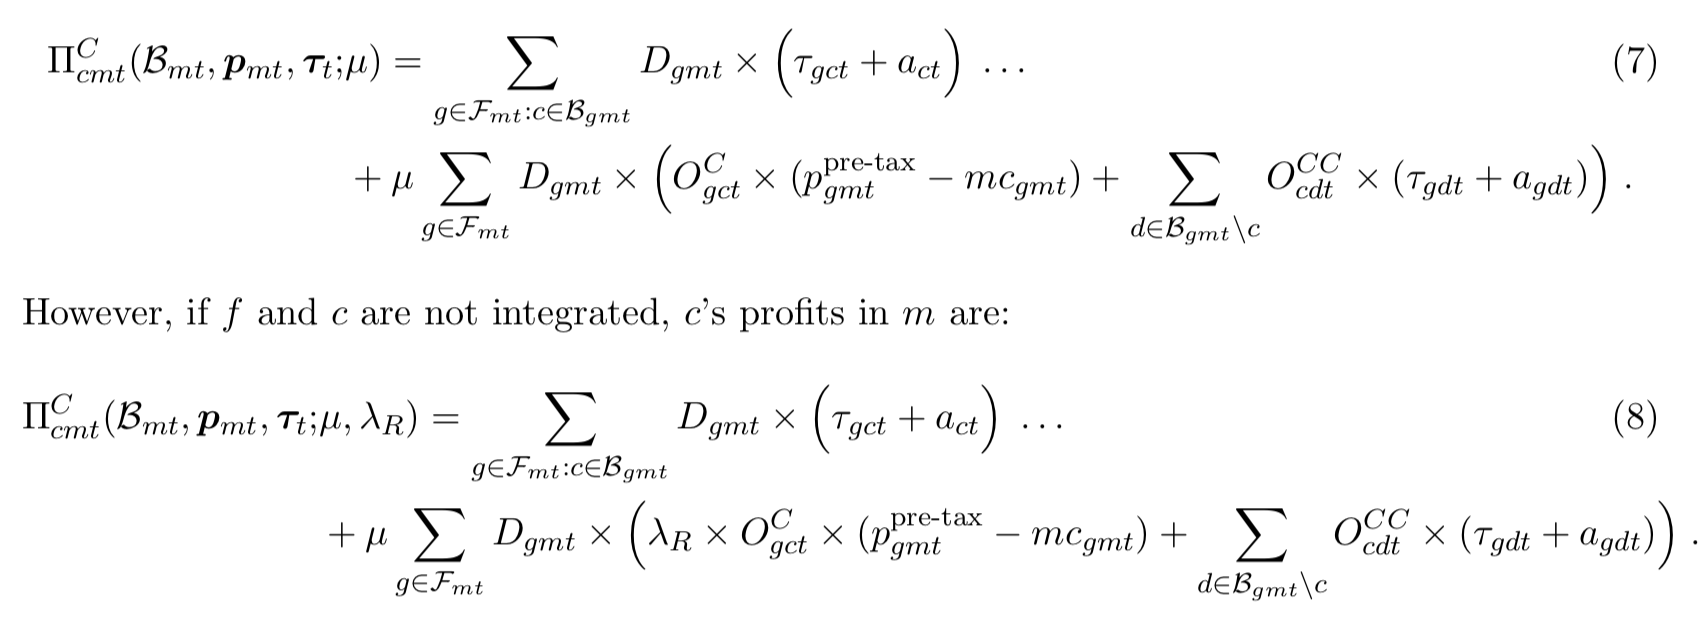
\includegraphics[width=4.5in]{./resources/mvpd1}
\end{center}
\begin{itemize}
\item Same as before $\mu$ is internalization of integrated profits
\item New parameter $\lambda_R$ is about \alert{raising rivals costs}.
\item Still get ad revenues but are different for channel and mvpd $a_{ct}$.
\end{itemize}

}

\frame[plain]{
\frametitle{Channel Payoffs / Bargaining}
\begin{center}
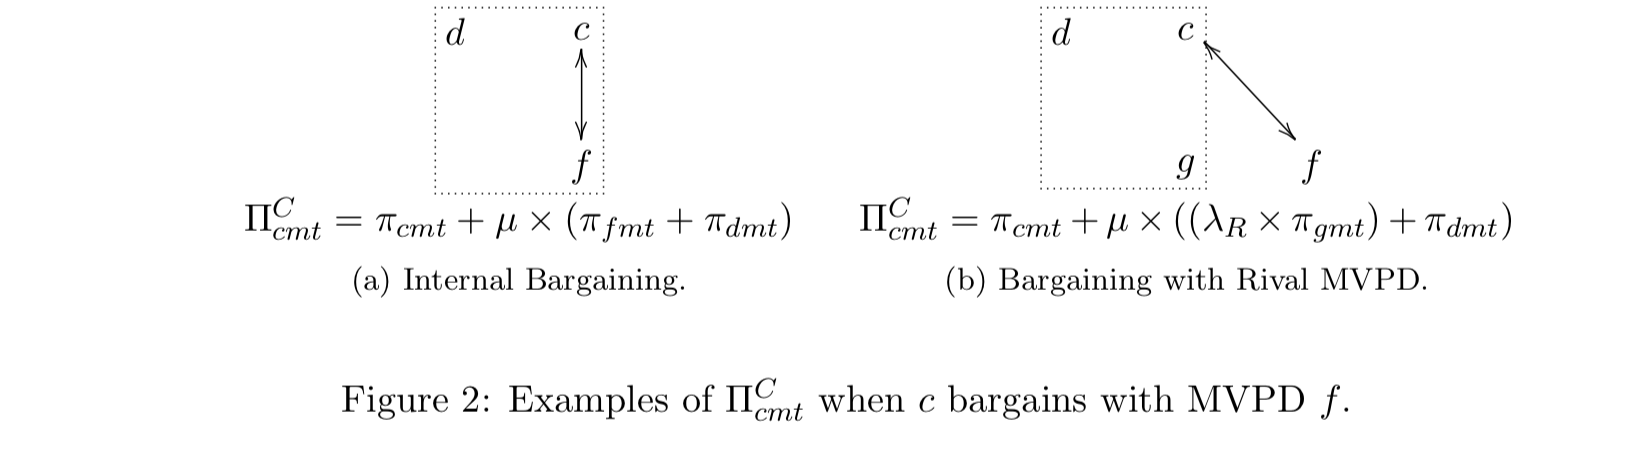
\includegraphics[width=5in]{./resources/mvpd2}
\end{center}
}


\frame[plain]{
\frametitle{Bargaining}
\begin{center}
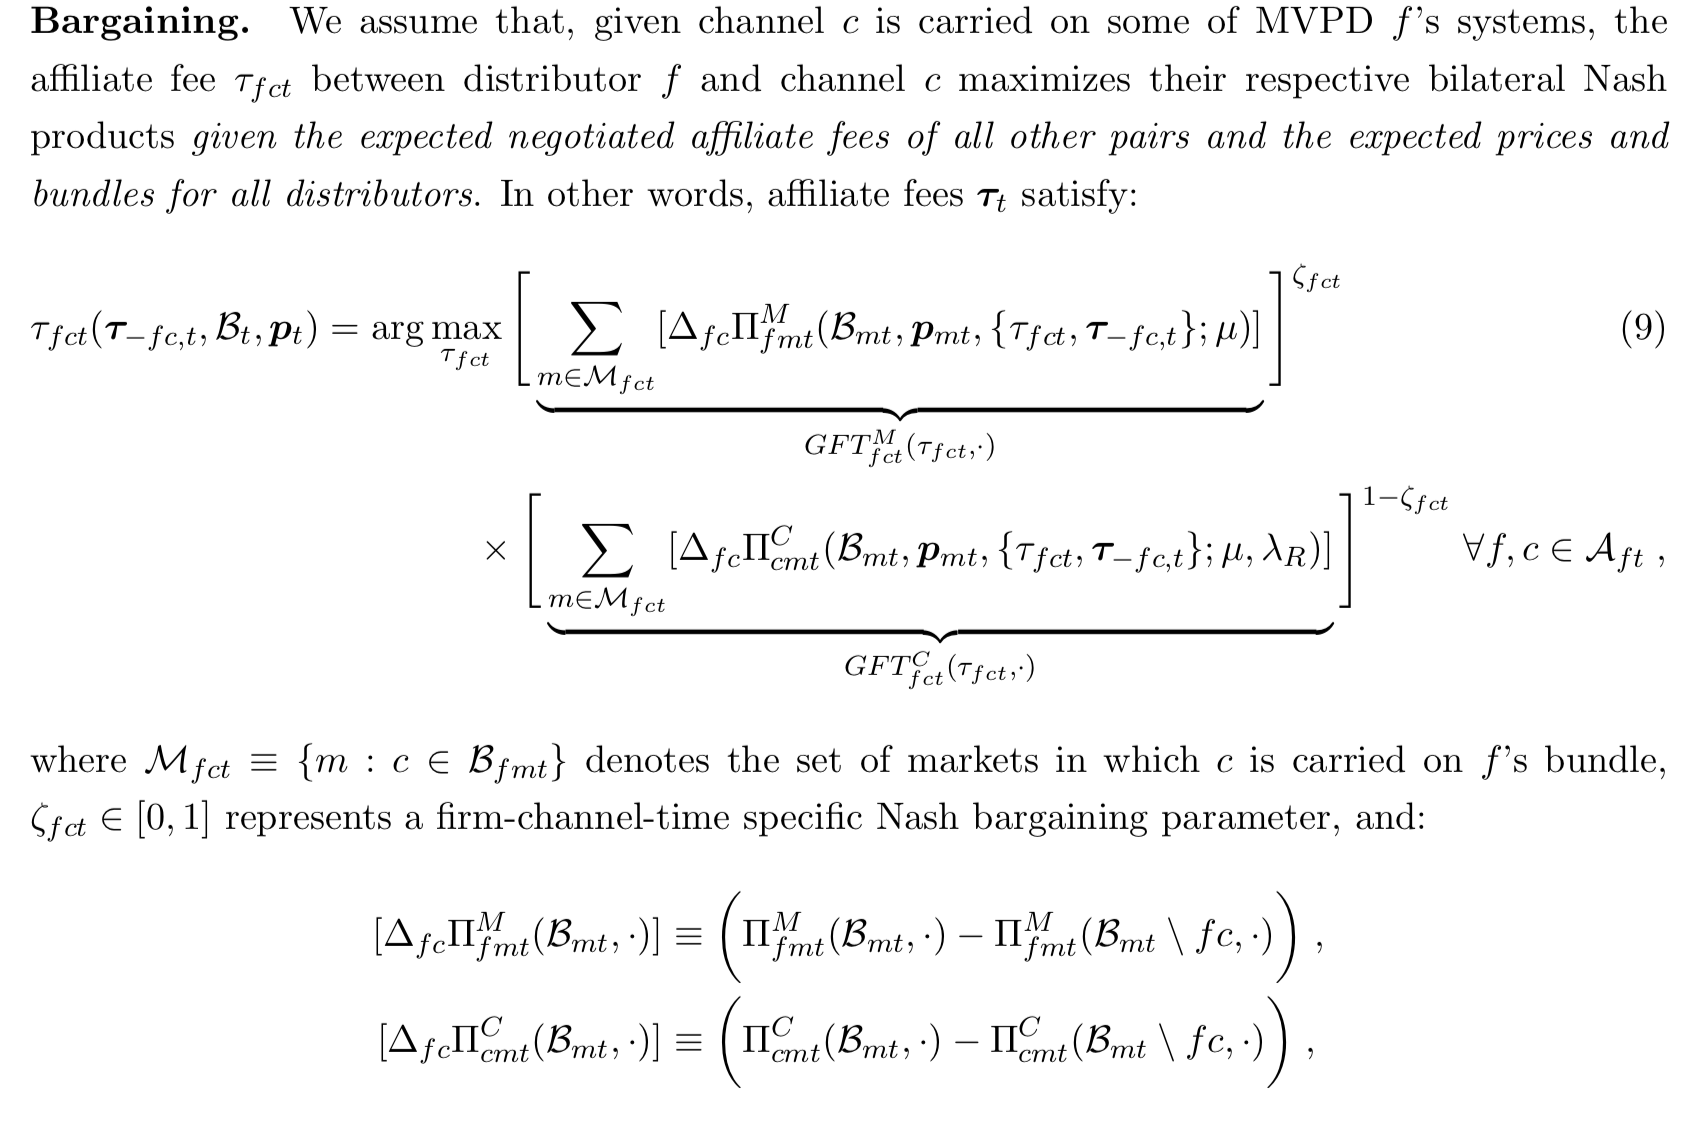
\includegraphics[width=4.5in]{./resources/mvpd3}
\end{center}
}

\frame[plain]{
\frametitle{Bargaining Example}
Ignore any vertical integration and think about just the bargaining:
\begin{center}
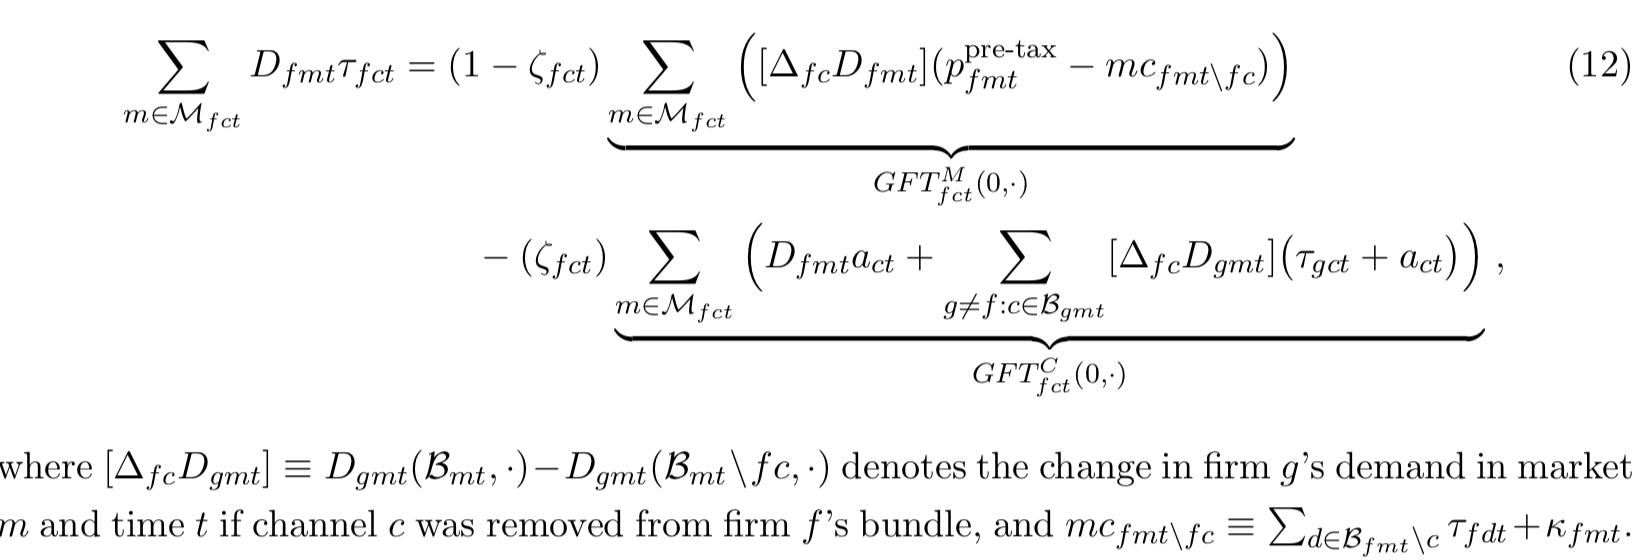
\includegraphics[width=4.5in]{./resources/mvpd4}
\begin{itemize}
\item Combined gains from trade from both $M$ and $C$
\item Last term is ``opportunity cost''.
\item Estimate two values for $\zeta \in \{\zeta^I, \zeta^E\}$.
\end{itemize}
\end{center}
}

\frame[plain]{
\frametitle{Nash in Nash Mechanics}
\begin{itemize}
\item Bargaining happens simultaneous with carriage and pricing
\item What this means is that if $\tau_{fct}$ changes then there is no change in $p_{fmt}$.
\begin{itemize}
\item Criticism is that this limits (but does not eliminate) mechanism for \alert{double marginalization} (by restricting what happens off the equilibrium path).
\item Sometimes criticized as ``schizophrenic'': division negotiating $\tau$ doesn't talk to local managers deciding $p_{fmt},\mathcal{B}_{fmt}$.
\end{itemize}
\item This is common in the literature: Grennan on Medical Devices, Ho or Ho and Lee on Hospitals-Insurers, Gowrisankaran, Nevo and Town on Hospitals-Insurers.
\item Collard-Wexler, Gowrisankaran and Lee (2017) attempt to micro-found the Nash-in-Nash solution.
\end{itemize}
}



\frame[plain]{
\frametitle{Double Marginalization}
Assume single channel $c$ fully owned by downstream firm $m$:
\begin{itemize}
\item Given $\tau$ firm $f$ sets the cable bundle price $p = \phi(mc_f + (1-\mu)\tau)$.
\begin{eqnarray*}
GFT_c^C(0,\cdot) &=&0  +  \mu \times (p - mc_f) D(p)\\
GFT_f^M(0,\cdot) &=& \mu \times (p - mc_f) D(p) + \mu \times 0
\end{eqnarray*}
\item The negotiated affiliate fee is then:
\begin{eqnarray*}
(1-\mu) \times D(p) = ( 1-\zeta)(p-mc_f) D(p) - \zeta \mu \times (p - mc_f) D(p)
\end{eqnarray*}
\item Holding $p$ fixed an increase in $\mu$ lowers $91-\mu)\tau$ (effective affiliate fee).
\item eq price satisfies $p = \phi(mc_f +[(1-\zeta) - \zeta \mu](p-mc_f))$.
\item Increasing $\mu$ lowers $p$.
\end{itemize}
}



\frame[plain]{
\frametitle{Identification}
\begin{center}
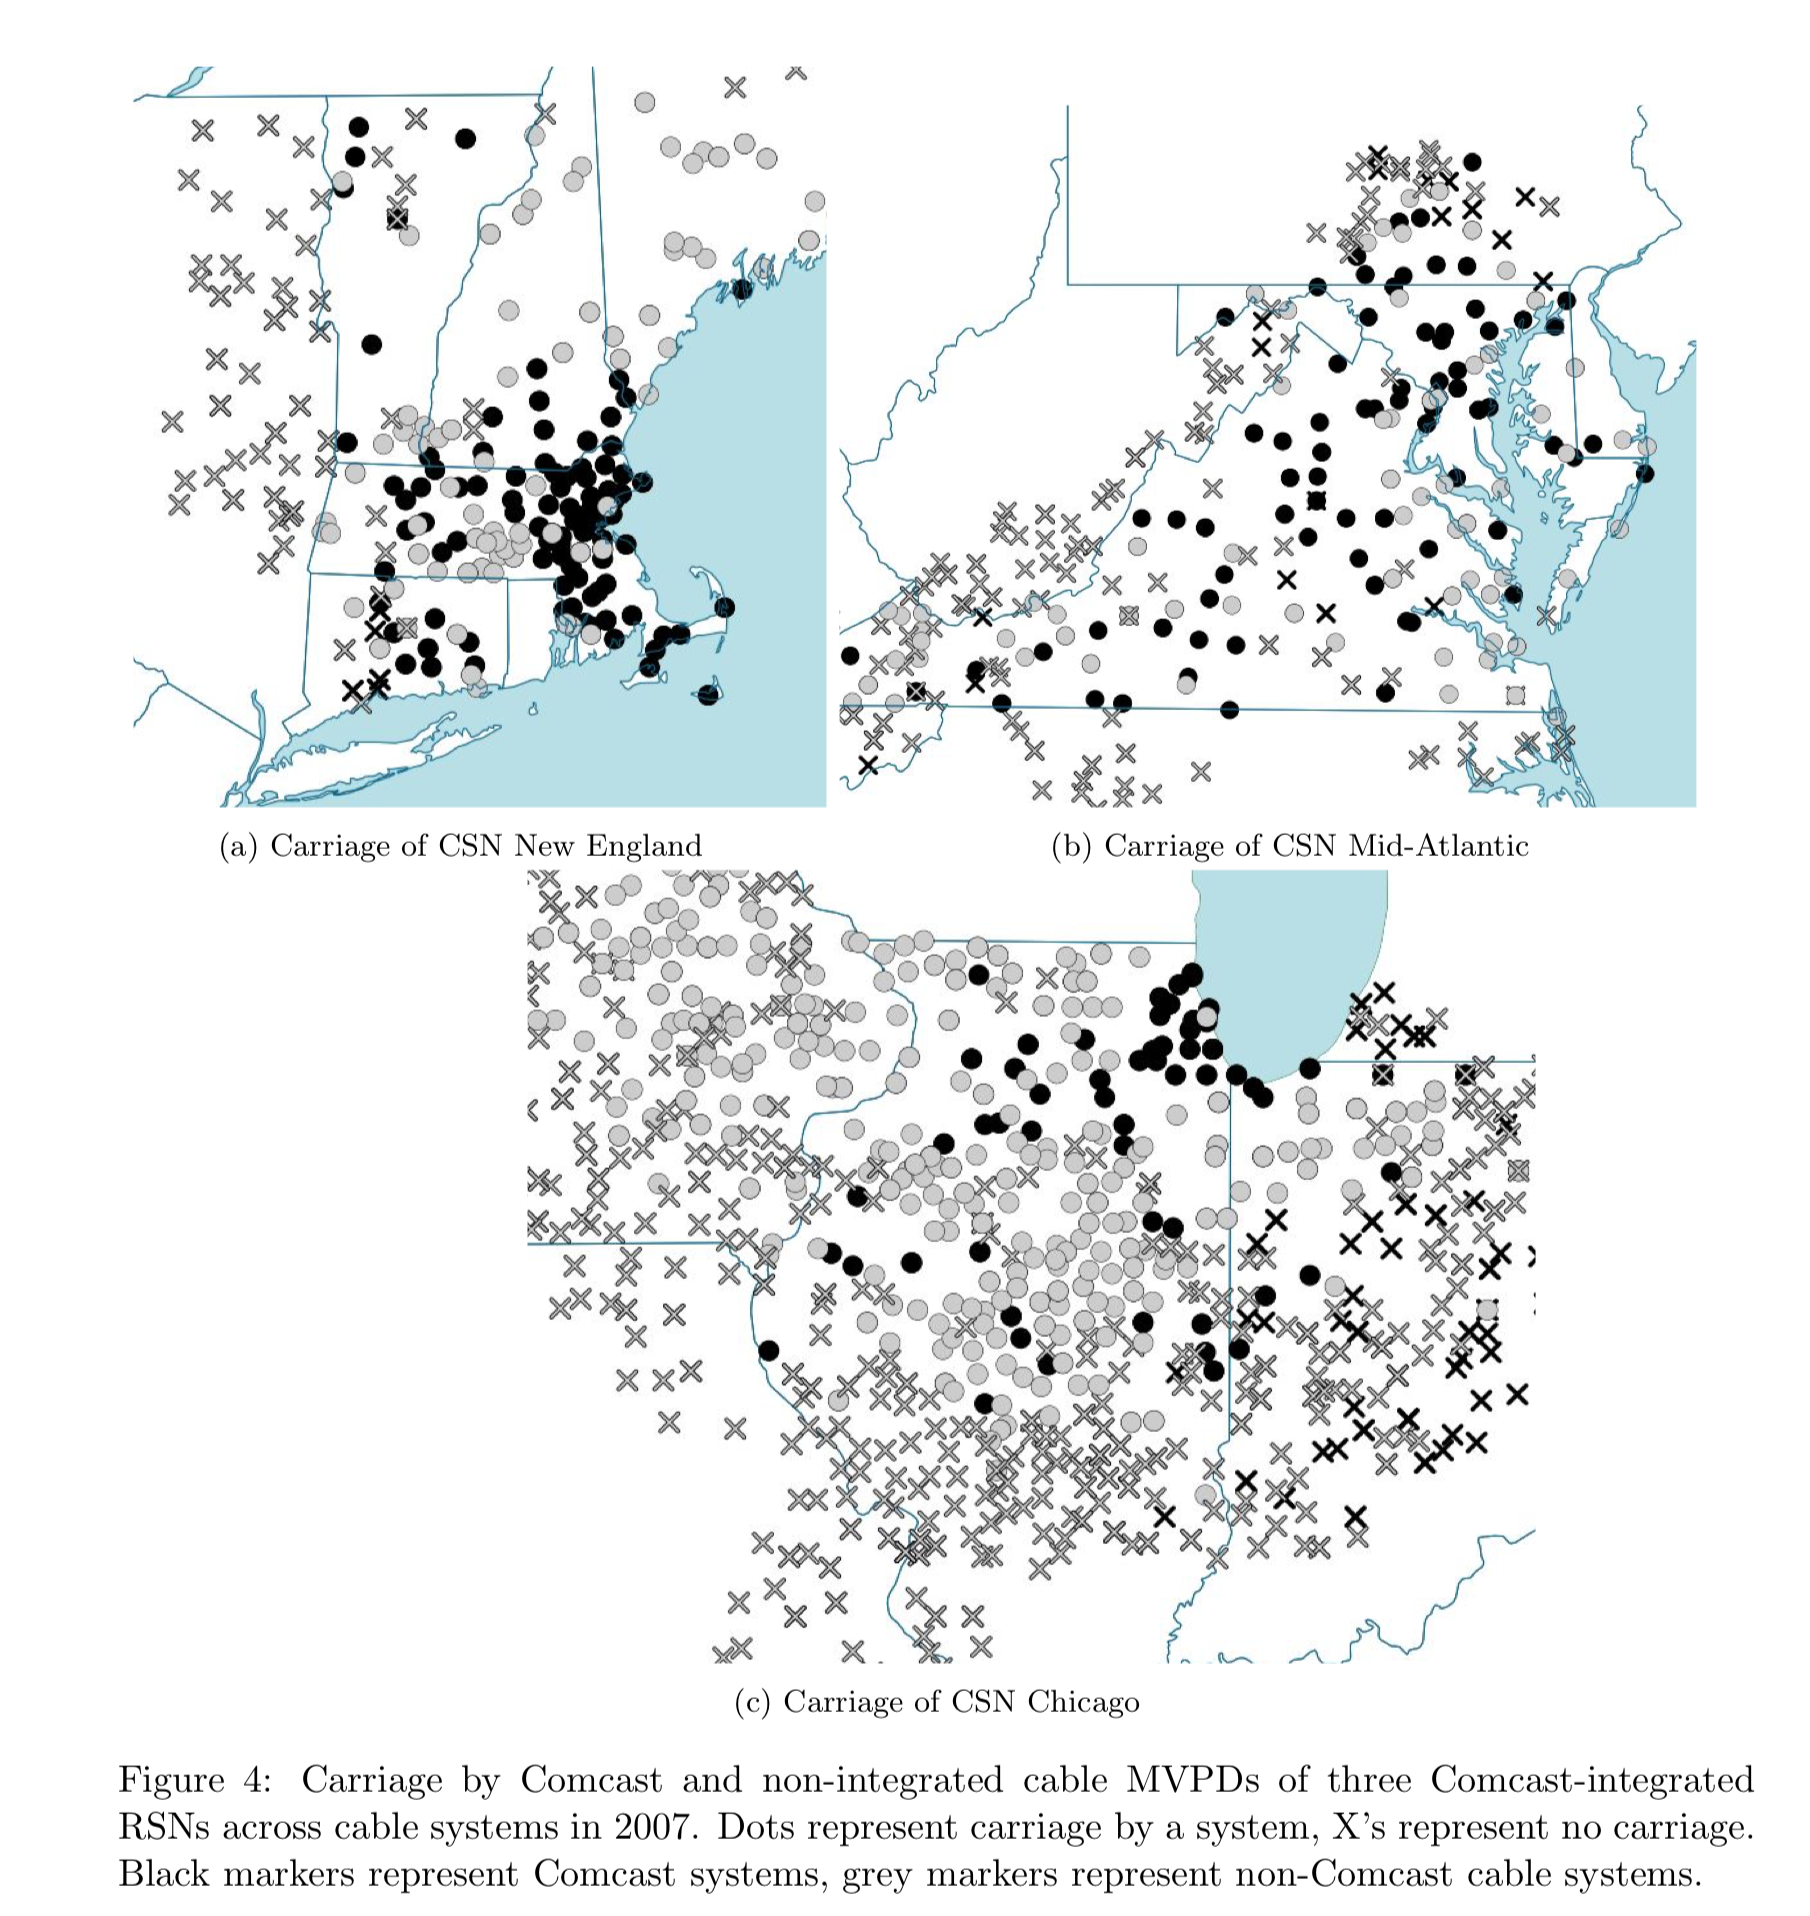
\includegraphics[width=3in]{./resources/mvpd5}
\end{center}
}

\frame[plain]{
\frametitle{  }
\begin{center}
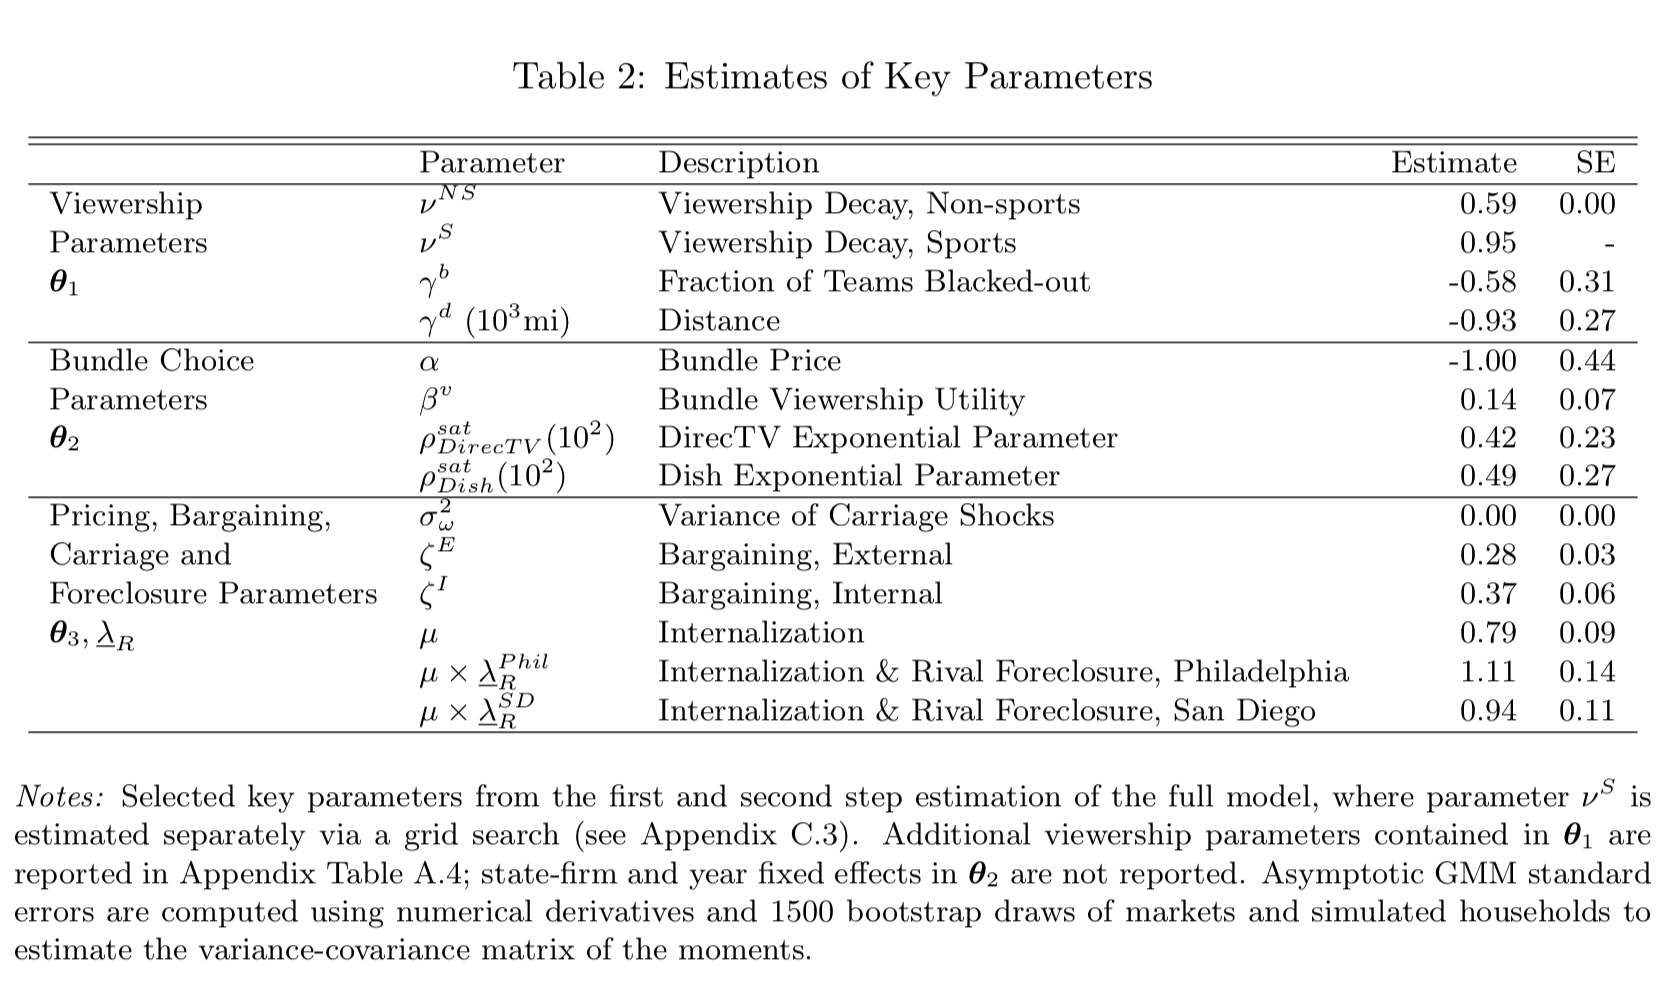
\includegraphics[width=4in]{./resources/mvpd6}
\end{center}
\begin{itemize}
\item Most markets have program access rules (PAR)s assume $\lambda_R = 0$.
\item Estimate lower bound on $\lambda_R$ because SAN and PHL have exclusion.
\end{itemize}
}

\begin{frame}{Results and Counterfactuals }
\begin{itemize}
\item Advantages of VI
\begin{itemize}
\item Lower negotiated price $\tau$ to cable company
\item Lower prices to consumers
\item More carriage by integrated firm
\end{itemize}
\item Disadvantages
\begin{itemize}
\item Higher prices to competitor (often satellite) $\tau$
\item Higher prices to competitor's customers $p$
\item Foreclosure or failure fo reach agreement.
\end{itemize}
\item Three scenarios
\begin{itemize}
\item No VI $(\mu=0)$.
\item VI with PARs $\lambda_R =0$
\item VI without PARs $\mu,\lambda_R$ both nonzero.
\end{itemize}
\end{itemize}
\end{frame}

\begin{frame}{Counterfactuals}
\begin{center}
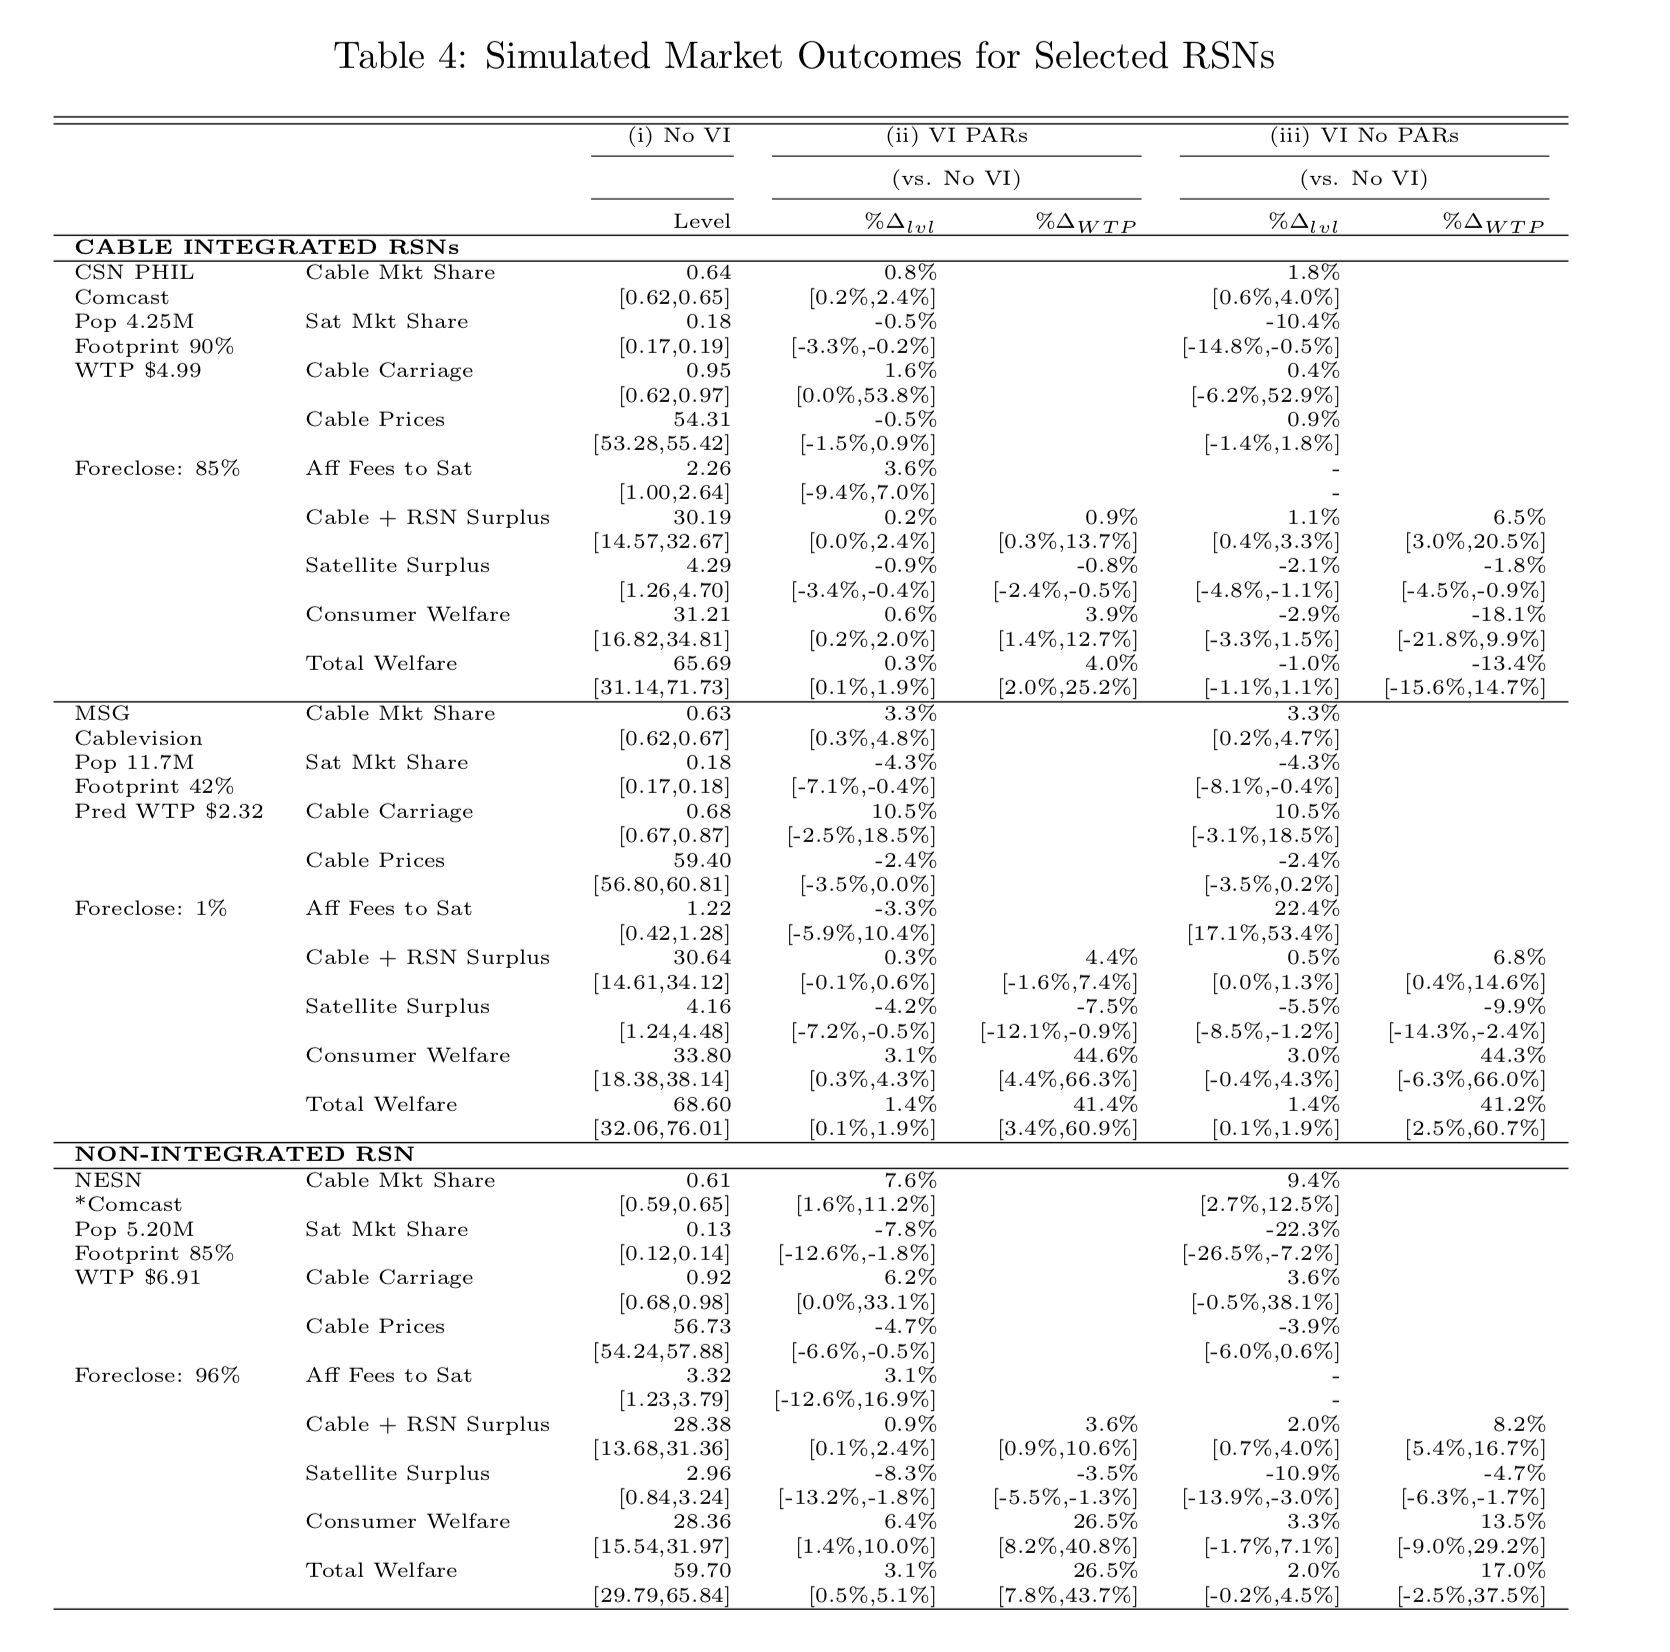
\includegraphics[width=3.25in]{./resources/mvpd7}
\end{center}
\end{frame}



\begin{frame}{Conclusions}
\begin{itemize}
\item VI is good but PARs are important.
\item Can we get the good without the bad simply by price discriminating
\begin{itemize}
\item ie: Charge a different price in Vermont than Boston for Celtics.
\end{itemize}
\end{itemize}
\end{frame}

\end{document}